%
% chapter.tex -- Topologie
%
% (c) 2025 Prof Dr Andreas Müller
%
\chapter{Topologie
\label{chapter:topologie}}
\kopflinks{Topologie}
%
% fig-torus.tex
%
% (c) 2025 Prof Dr Andreas Müller
%
\begin{figure}
\centering
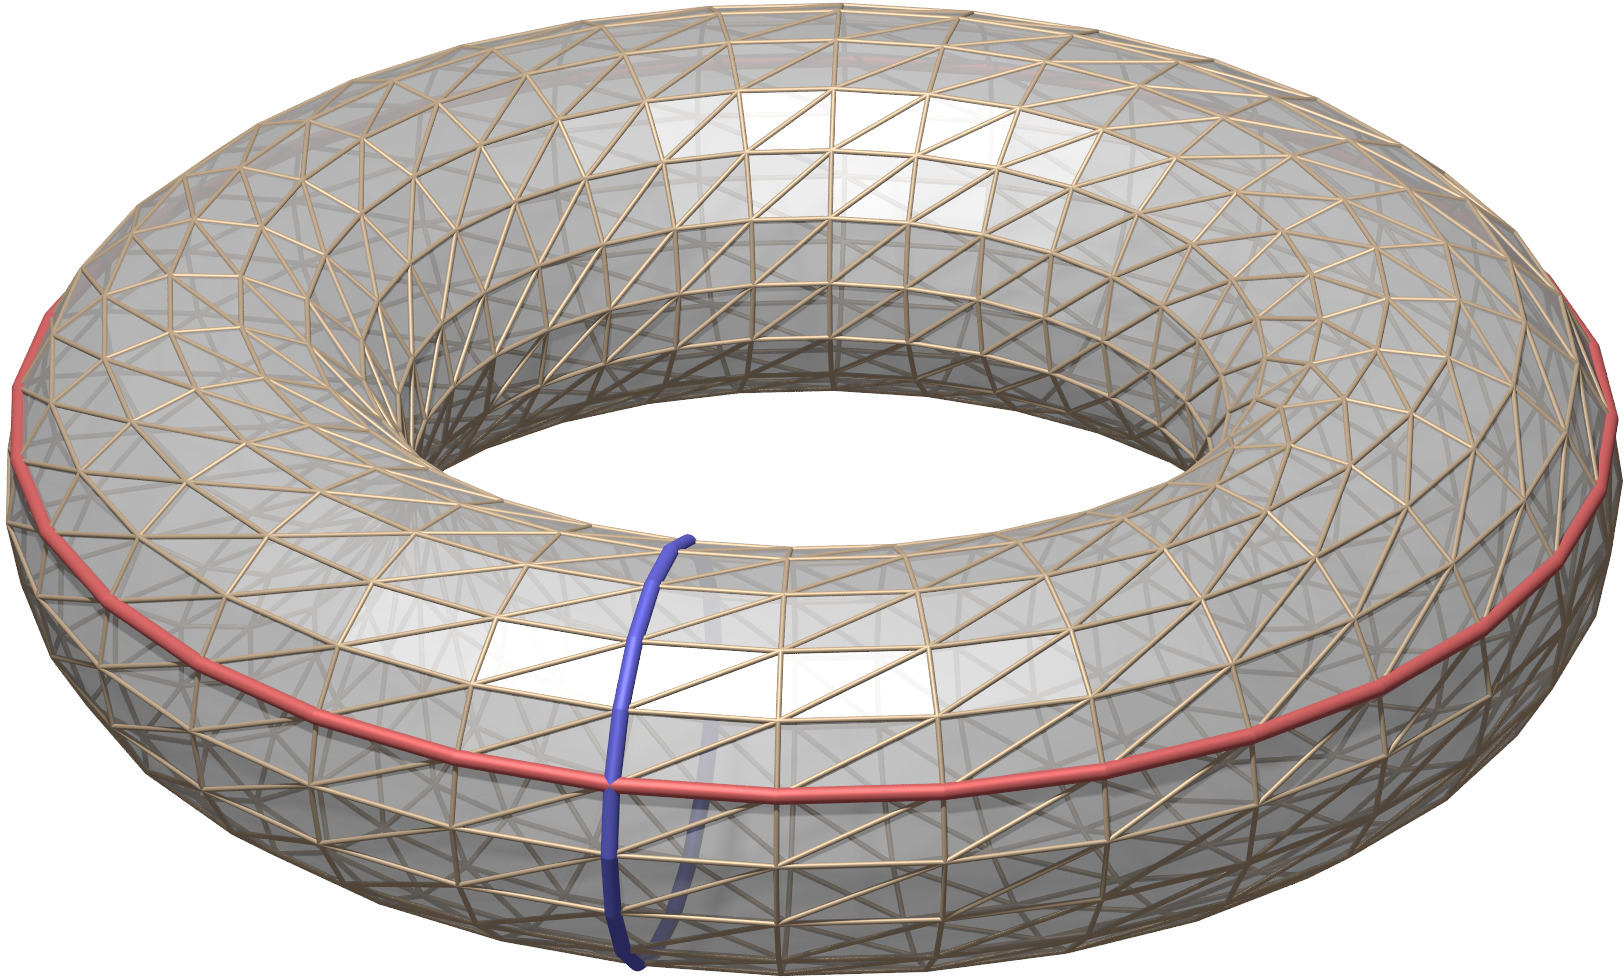
\includegraphics[width=\textwidth]{chapters/120-topologie/images/torus.jpg}
\caption{Triangulation eines Torus mit 576~Ecken, 1728~Kanten und
1152~Dreiecken.
Der Torus hat daher die Euler-Charakteristisk $0$.
\label{buch:topologie:intro:fig:torus}}
\end{figure}
%
%
% fig-sphaere.tex
%
% (c) 2025 Prof Dr Andreas Müller
%
\begin{figure}
\centering
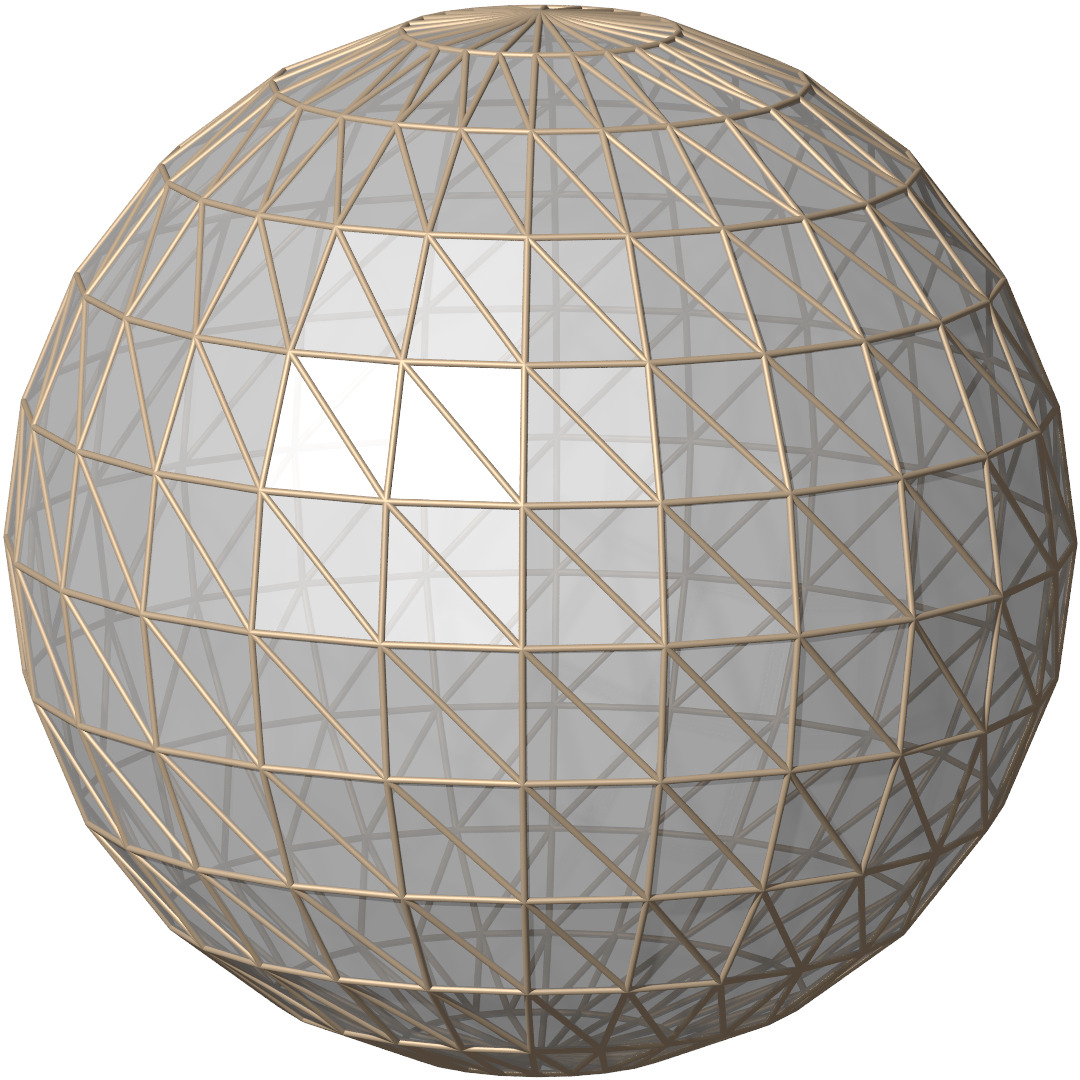
\includegraphics[width=0.6\textwidth]{chapters/120-topologie/images/sphaere.jpg}
\caption{Triangulation einer Kugel mit 266~Ecken, 792~Kanten und
528~Dreiecken.
Die Kugel hat daher die Euler-Charakteristisk $2$.
\index{Kugel}%
\index{Triangulation}%
\label{buch:topologie:intro:fig:sphere}}
\end{figure}
%
%
% table-polyeder.tex
%
% (c) 2025 Prof Dr Andreas Müller
%
\begin{table}
\centering
\begin{tabular}{l>{$}r<{$}>{$}r<{$}>{$}r<{$}>{$}r<{$}}
\hline
Polyeder          &\text{Ecken}&\text{Kanten}&\text{Flächen}&\chi(M)\\
\hline
Tetraeder         &           4&            6&             4&      2\\
Oktaeder          &           6&           12&             8&      2\\
Hexader (Würfel)  &           8&           12&             6&      2\\
Dodekaeder        &          20&           30&            12&      2\\
Ikosaeder         &          12&           30&            20&      2\\
\hline
Kugel             &         266&          792&           528&      2\\
Torus             &         576&         1728&          1152&      0\\
\hline
\end{tabular}
\caption{Die eulerschen Polyeder haben alle die Euler-Charakteristik $2$.
Während die Triangulation einer Kugel aus
\index{Euler-Charakteristik}%
\index{Tetraeder}%
\index{Oktaeder}%
\index{Hexaeder}%
\index{Würfel}%
\index{Dodekaeder}%
\index{Ikosaeder}%
Abbildung~\ref{buch:topologie:intro:fig:sphere} wie die Polyeder
Euler-Charakteristik $2$ hat, ergibt die Triangulation des Torus von
\index{Triangulation}%
Abbildung~\ref{buch:topologie:intro:fig:torus} jedoch
der Wert 0, der zum Ausdruck bringt, dass der Torus ein ``Loch''
\index{Torus}%
\index{Kugel}%
hat.
\label{buch:topologie:intro:table:eulercharakteristik}}
\end{table}
%

\noindent
Das Poincaré-Lemma ist der erste Hinweis darauf, dass die grossräumige
Gestalt einer Mannigfaltigkeit einen Einfluss darauf hat, ob sich eine
Differentialgleichung lösen lässt.
Es sagt nämlich, dass es auf einer zusammenziehbaren Mannigfaltigkeit
immer eine Lösung der Gleichung $d\alpha = 0$ im Raum der $p$-Formen
gibt.
Die Kohomologie-Theorie vertieft diese Idee und definiert eine Familie
von Vektorräumen, deren Dimension angibt, wieviele in noch zu definierendem
Sinn wesentlich verschiedene Lösungen eine solche Gleichung haben kann.
Diese Dimensionszahlen geben wesentliche Informationen über die grossräumige
Gestalt der Mannigfaltigkeit.

Auf Leonhard Euler geht die Beobachtung zurück, dass für ein beliebiges
geschlossenes Polyeder ohne Löcher im Raum immer
\begin{equation}
\#\{\text{Ecken}\}
-
\#\{\text{Kanten}\}
+
\#\{\text{Flächen}\}
=
E-K+F
=
2
\label{buch:topologie:eqn:eulerpolyeder}
\end{equation}
gilt.
Da sich eine beliebige zweidimensionale Mannigfaltigkeit triangulieren
lässt, kann diese Zahl auch für eine Triangulierung berechnet werden.
Es stellt sich heraus, dass 
die Zahl \eqref{buch:topologie:eqn:eulerpolyeder}
nicht von der Triangulierung abhängt und sich auch aus den Dimensionszahlen
der Kohomologievektorräume berechnen lässt.
Sie heisst heute die Euler-Charakteristik $\chi(M)$ einer Mannigfaltigkeit.
Tabelle~\ref{buch:topologie:intro:table:eulercharakteristik} enthält
eine Zusammenstellung der Euler-Charakteristiken der eulerschen Polyeder
sowie von Triangulationen von Torus und Kugel.

Das Gebiet der algebraischen Topologie befasst sich genau mit dieser Art
der Beschreibung der ``Gestalt'' von topologischen Räumen.
Für Mannigfaltigkeiten stellt sie einen besonders vielfältigen
Werkzeugkasten bereit, der solche Fragestellungen sowohl mit
kombinatorischen wie auch mit analytischen Aspekten einer Mannigfaltigkeit
verbinden kann.
Ziel dieses Kapitels ist, einen Ausblick auf die wichtigsten Ideen
dieser reichhaltigen Theorie zu geben.

%
% Euler-Charakteristik
%
\section{Euler-Charakteristik}
Die von Euler entdeckte kombinatorische Eigenschaft der platonischen
Körper lässt sich auf beliebige triangulierte Körper und sogar
auf Mannigfaltigkeiten höherer Dimension ausdehnen.
Die Vorgehensweise und die wichtigsten Eigenschaften sollen in den
folgenden Abschnitten skizziert werden.

%
% Triangulationen
%
\subsection{Triangulationen}
Eine Triangulation einer Fläche zerlegt die Fläche in Dreiecke,
Kanten und Punkte.
Dabei müssen Ecken und Kanten von benachbarten Dreiecken aufeinander
fallen.
Es ist zum Beispiel nicht zulässig, dass eine Ecke eines Dreiecks
auf einen inneren Punkt einer Kante eines Nachbardreiecks fällt.

%
% Simplizes
%
\subsubsection{Simplizes}
Punkte, Kanten und Dreieck sind die vertraute Spezialfälle des allgemeinen
Konzeptes eines Simplex.

\begin{definition}[Simplex]
\index{Simplex}%
Ein \emph{$n$-dimensionales Simplex} ist die Menge
\[
\Delta_n
=
\{
(t_0,\dots,t_n)
\subset
[0,1]^{n+1}
\mid
t_0+\dots+t_n=1
\}.
\]
\end{definition}

Im Falle $n=0$ besteht $\Delta_0$ nur aus der Zahl $1$.
$\Delta_1$ besteht aus Paaren $(t_0,t_1)$ mit $t_0+t_1=1$, die
als die Strecke zwischen $(1,0)$ und $(0,1)$ visualisiert
werden.
Ebenso besteht die Menge $\Delta_2$ aus den Punkten der Ebene mit
der Gleichung $t_1+t_2+t_3=1$ im postiven Oktanten eines
dreidimensionalen kartesischen Koordinatensystems mit Koordinaten
$t_1$, $t_2$ und $t_3$.

In der Teilmenge
\[
\Delta_{n,i}
=
\{
(t_0,\dots,t_n)
\subset
[0,1]^{n+1}
\mid
t_0+\dots+t_n=1
\wedge
t_i=0
\}
\subset
\Delta_n
\]
sind $n+1$-Tupel, deren $i$-Koordinate verschwindet.
Die Mengen $\Delta_{n,i}$ heissen die \emph{Seitenflächen}
\index{Seitenfläche}%
des Simplex $\Delta_n$.

Für die verbleibenden Koordinaten gilt wegen $t_i=0$ ebenfalls
\[
t_0+\dots+t_i+\dots+t_n
=
t_0+\dots+\widehat{t_i}+\dots+t_n
=
1,
\]
Wobei der Hut bedeutet, dass dieser Term weggelassen wird.
Man kann die Menge also durch die Abbildung
\[
\iota_i
\colon
\Delta_{n-1}
\to
\Delta_{n,i}
:
(t_0,\dots,t_{n-1})
\mapsto
(t_0,\dots,0,\dots,t_{n-1})
\]
parametrisieren.
Die Abbildung $\iota_i$ ist bijektiv, stetig und die Umkehrung ist
ebenfalls stetig.
Die Seitenflächen $\Delta_{n,i}$ sind also Simplizes kleinerer 
Dimension.

Zwei Seitenflächen stossen zusammen in einer Menge, die ein Simplex
der Dimension $n-2$ ist.
Die gemeinsamen Punkte der beiden Seitenflächen $\Delta_{n,i}$ und
$\Delta_{n,k}$ bilden die Menge
\[
\Delta_{n,ik}
=
\{
(t_0,\dots,t_n)
\mid
t_0+\dots+t_n=1
\wedge
t_i=0
\wedge
t_k=0
\},
\]
die sich nach dem gleichen Muster wie die Seitenfläche mit der Menge
$\Delta_{n-2}$ identifizieren lässt.

\begin{definition}[simplizialer Komplex]
\index{simplizialer Komplex}%
Ein \emph{simplizialer Komplex} ist ein topologischer Raum, der durch
Zusammenfügen von endlich vielen Simplizes entlang von Untersimplizes
kleinerer Dimension entsteht.
\index{Dimension}%
Die \emph{Dimension} eines simplizialen Komplexes ist die höchste Dimension
der Simplizes, aus denen er besteht.
\end{definition}

Ein simplizialer Komplex der Dimension $n$ setzt sich also zusammen aus
maximal $n$-dimensionalen Simplizes zusammen, die Seitenflächen oder
Simplizes noch kleinerer Dimension gemeinsam haben können.

%
% Euler-Charakteristik einer Triangulation
%
\subsubsection{Euler-Charakteristik eines simplizialen Komplexes}
Eulers Entdeckung bezog sich auf Polyeder, die sich natürlich nur
aus Ecken, Kanten und Flächen, also Simplizes der Dimension 0, 1
bzw.~2.
Bezeichnen wir die Anzahl der $k$-dimensionalen Simplizes mit $t_k$,
dann wird die von Euler berachtete Summe 
\begin{align*}
E - K + K
&=
t_0
-
t_1
+
t_2
\intertext{Die wir auch}
&=
\sum_{k=0}^2 (-1)^kt_k
\end{align*}
schreiben können.
Diese Schreibweise lässt sich leicht auf beliebige Dimension
verallgemeinern.

\begin{definition}[Euler-Charakteristik]
Sei $S$ ein $n$-dimensionaler simplizialer Komplex in dem
genau $k_i$ Simplizes der Dimension $i$ vorkommen.
Dann ist die Summe
\[
\chi(S)
=
k_0 - k_1 + \dots + (-1)^n t_n
=
\sum_{i=0}^n (-1)^i k_i
\]
die \emph{Euler-Charakteristik} von $S$.
\index{Euler-Charakteristik}%
\end{definition}

%
% Verfeinerung der Triangulation
%
\subsubsection{Verfeinerung der Triangulation}
Die Definition der Euler-Charakteristik hängt von der Triangulation ab.
Wir müssen daher zeigen, dass eine Verfeinerung der Triangulation die
Euler-Charakteristik nicht ändert.
Statt eines vollständigen Beweises dieser Eigenschaft zeigen wir anhand
einiger illustrativer Beispiele, was sich bei der Verfeinerung
abspielt.
%
% fig-unterteilung.tex
%
% (c) 2025 Prof Dr Andreas Müller
%
\begin{figure}
\centering
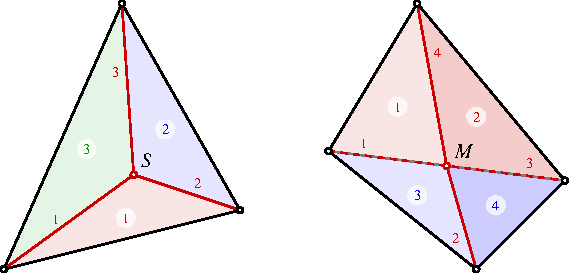
\includegraphics{chapters/120-topologie/images/unterteilung.pdf}
\caption{Links: Bei der Unterteilung eines einzelnen Dreiecks durch einen
inneren Punkt $S$ entstehen drei Dreieck ($2$ mehr also vor der Unterteilung)
und 3 neue Kanten.
Rechts: Bei der Unterteilung der Kante $AB$ durch den Punkt $M$ werden
\index{Unterteilung}%
beide Nachbardreiecke (rot und blau) in jeweils zwei Dreiecke
($2$ mehr als vor der Unterteilung)$ zerlegt.
Ausserdem entstehen drei zusätzliche Kanten.
In allen Fällen ändert sich die Euler-Charakteristik nicht.
\label{buch:topologie:eulercharakteristik:fig:unterteilung}}
\end{figure}
%

Wir beginnen mit einer triangulierten zweidimensionalen Mannigfaltigkeit
und betrachten ein einzelnes Dreieck.
Die Triangulation kann verfeinert werden, indem im Inneren des
Dreiecks ein weiterer Punkt hinzugefügt wird
(Abbildung~\ref{buch:topologie:eulercharakteristik:fig:unterteilung} links).
Neue Kanten vom neuen Punkt zu den Ecken des Dreiecks ergeben die
verfeinerte Triangulation.
Die Triangulation bekommt also eine zusätzliche Ecke, drei zusätzliche
Kanten und aus einem Dreieck werden drei, also zwei zusätzliche Dreiecke.
Für die Euler-Charakteristik bekommen wir daher
\[
(E+1) - (K+3) - (F+2)
=
E-K+F+(\underbrace{1-3+2}_{\displaystyle=0})
=
E-K+F,
\]
die Euler-Charakteristik ändert also nicht.

Unterteilt man eine Kante mit einem neuen Punkt, dann müssen auch
die angrenzenden beiden Dreiecke mit einer Kante zur gegenüberliegenden
Ecke neu unterteilt werden
(Abbildung~\ref{buch:topologie:eulercharakteristik:fig:unterteilung} rechts).
Die Anzahl der Ecken vergrössert sich um eins.
Aus der ursprünglichen Kante werden zwei und es kommen zwei neue Kanten
dazu.
Die Anzahl der Dreiecke wächst um zwei.
Die Euler-Charakteristik ist neu
\begin{align*}
(E+1) - (K+3) - (F+2)
=
E-K+F +(\underbrace{1-3+2}_{\displaystyle=0})
=
E-K+F,
\end{align*}
sie verändert sich also auch bei Unterteilung einer Kante nicht.

In drei Dimensionen wird die Unterteilung etwas komplizierter.
Ein zusätzlicher innerer Punkt in einem Tetraeder zerlegt
es in vier Tetraeder mit dem neuen Punkt als Spitze und den
Seitenflächen des ursprünglichen Tetraeders als Grundfläche.
Für jede ursprüngliche Kante entsteht eine neue Fläche und
für jede ursprüngliche Ecke eine neue Kante.
Die Euler-Charakteristik wird daher zu
\begin{align*}
(E+1) - (K+4) + (F+6) - (V+3)
&=
E-K+F-V
+
(\underbrace{1-4+6-3}_{\displaystyle=0})
\\
&=
E-K+F-V
=
\chi(M),
\end{align*}
bleibt daher unverändert.

Unterteilt man eine Dreiecksfläche durch einen inneren Punkt,
müssen auch die beiden benachbarten Tetraeder unterteilt werden.
Dabei entstehen fünf neue Kanten, sechs neue Flächen und vier
neue Tetraeder.
Die neue Euler-Charakteristik ist daher
\begin{align*}
(E+1) - (K+5) + (F+8) - (V+4)
&=
E-K+F-V
+(\underbrace{1-5+8-4}_{\displaystyle=0})
\\
&=
E-K+F-V
=
\chi(M),
\end{align*}
ebenfalls unverändert.

Schliesslich betrachten wir den Fall der Unterteilung einer Kante,
die $n$ Tetraedern gemeinsam ist, mit $f$ Seitenflächen, die sich
in der Kante treffen.
Durch die Unterteilung wird aus jeder Seitenfläche zu zweien
mit einer zusätzlichen Kante.
Zusätzlich entsteht in jedem ursprünglichen Tetraeder ein zusätzliches
Dreieck mit der gegenüberliegenden Kante als Basis und der neuen
Ecke als Spitze.
Die Zahl der Tetraeder erhöht sich ebenfalls um $n$.
Die neue Euler-Charakteristik ist
\begin{align*}
(E+1)
-
(K+1+f)
+
(F+f+n)
-
(V+n)
&=
E-K+F-V + (\underbrace{1-1-f+f+n-n}_{\displaystyle=0})
\\
&=
E-K+F-V
=
\chi(M),
\end{align*}
wieder unverändert.

Dieselbe Art von Rechnung lässt sich auch für Simplizes beliebig hoher
Dimension durchführen.
Ohne auf den detaillierten Beweis einzugehen, können wir schliessen,
dass die Euler-Charakteristik eine Grösse ist, die nicht von der Unterteilung
des Körpers in Simplizes abhängt.
Die Euler-Charakteristik ist also eine topologische Invariante.

%
% Rand
%
\subsubsection{Rand}


%
% Homologie
%
\subsection{Homologie}

\subsubsection{Vektorraum der Simplizes}
Der Rand eines Simplexes ist nicht ein einzelnes Simplex, sondern
eine Menge von Simplizes.
Genau genommen müssen wir ausserdem auch noch die Orientierung eines
Simplexes berücksichtigen.
Ein zweidimensionales Simplex mit den Ecken $ABC$ hat als Rand
die drei Simplizes $AB$, $BC$ und $AC$, aber das letzte wird in
entgegengesetzter Richtung durchlaufen.

\begin{definition}
Sei $S$ ein $n$-dimensionaler simplizialer Komplex.
Für jedes $k$, $0\le k\le n$ ist $C_k$ der reelle Vektorraum, aufgespannt
von den Simplizes von $S$.
\end{definition}



\begin{beispiel}
\label{buch:topologie:eulercharakteristik:bsp:dreieck}
Wir betrachten den simplizialen Komplex, der aus nur einem Dreieck
$\triangle ABC$ besteht.
Die $0$-dimensionalen Simplizes sind die Ecken $A$, $B$ und $C$, 
die eindimensionalen Simplizes sind die Kanten $AB$, $BC$ und $AC$.
Deher sind die Vektorräume
\begin{align*}
C_0 &= \{ x_A A + x_B B + x_C C\mid x_A, x_B, x_C\in\mathbb{R}\}
&
\dim C_0 &= 3 \\
\\
C_1 &= \{ x_{AB} AB + x_{BC} BC + x_{AC} AC\mid x_{AB}, x_{BC}, x_{AC} \in\mathbb{R}\}
&
\dim C_1 &= 3 \\
\\
C_2 &= \{ x_{ABC} ABC\mid x_{ABC}\in\mathbb{R}\}
&
\dim C_2 &= 1
\end{align*}
\end{beispiel}

%
% Randoperator
%
\subsubsection{Randoperator}
Da wir jetzt beliebige Simplizes linear kombinieren können, können
wir auch den Rand eines Simplex als Linearkombination von nideriger
dimensionalen Simplizes ausdrücken.

\begin{definition}[Randoperator]
Der $k$-dimensionale Randoperator ist die lineare Abbildung
\[
\partial_k
\colon
C_k \to C_{k+1}
:
P_0\dots P_k
\mapsto
\sum_{i=0}^k
(-1)^i
P_0\dots\widehat{P_i}\dots P_k.
\]
\index{Randoperator}%
\end{definition}

\begin{beispiel}
Das Beispiel~\ref{buch:topologie:eulercharakteristik:bsp:dreieck}
konstruiert die Vektorräume $C_k$ für ein Tetraeder.
Der $0$-dimensionale Randoperator $\partial_0$ ist der Null-Operator.
In höheren Dimension sind Randoperatoren
\begin{align*}
\partial_1 AB &= -B + A \\
\partial_1 BC &= -C + B \\
\partial_1 AC &= -C + A \\
\partial_2 ABC &= AB - AC + BC
\end{align*}
\end{beispiel}

\begin{satz}
Der Rand eines Randes verschwindet, $\partial_{k-1}\circ\partial_k=0$.
\end{satz}

\begin{proof}
Da der Randoperator linear ist, muss die Behauptung nur auf $k$-dimensionalen
Simplizes verifiziert werden.
Sei also $\sigma=P_0\dots P_k$ ein $k$-dimensionales Simplex.
Der Randoperator ergibt
\[
\partial_k\sigma
=
\sum_{i=0}^k
(-1)^i P_0\dots\widehat{P_i}\dots P_k.
\]
Die Summanden sind $k-1$-dimensionale Simplizes, deren Rand wir jetzt
zusätzlich ausrechnen müssen.
Dabei müssen erneut Punkte $P_j$ weggelassen und mit einem Vorzeichen versehen
werden.
Da das Vorzeichen von der Position und nicht vom Index abhängt, unterscheiden
wird die Fälle $j<i$ und $j>i$:
\begin{align*}
\partial_{k-1}\partial_k \sigma
&=
\sum_{i=0}^k (-1)^i \partial_{k-1} P_0\dots \widehat{P_i}\dots P_k
\\
&=
\sum_{i=0}^k
\biggl(
\sum_{j=0}^{i-1}
(-1)^{i+j}P_0\dots\widehat{P_j}\dots \widehat{P_i}\dots P_k
+
\sum_{j=i+1}^{k}
(-1)^{i+j+1}P_0\dots\widehat{P_i}\dots \widehat{P_j}\dots P_k
\biggr)
\\
&=
\sum_{j<i}
(-1)^{i+j}P_0\dots\widehat{P_j}\dots \widehat{P_i}\dots P_k
+
\sum_{i<j}
(-1)^{i+j+1}P_0\dots\widehat{P_i}\dots \widehat{P_j}\dots P_k.
\intertext{Vertauschen wir die Namen der Summationsvariablen in der
zweiten Summe und verwandeln wird den Summanden $+1$ im Exponenten
in ein Vorzeichen vor der Summe, entsteht}
&=
\sum_{j<i}
(-1)^{i+j}P_0\dots\widehat{P_j}\dots \widehat{P_i}\dots P_k
-
\sum_{j<i}
(-1)^{i+j}P_0\dots\widehat{P_j}\dots \widehat{P_i}\dots P_k.
\end{align*}
Die beiden Summen heben sich weg, was die Behauptung beweist.
\end{proof}

%
% Zyklen und Ränder
%
\subsubsection{Zyklen und Ränder}
Der Randoperator ist ein linearer Operator und wird daher wesentlich
durch Kennzahlen wie Rang und Dimension des Kernes charakterisiert.
Wir geben Kern und Bild des Randoperators spezielle Namen.

\begin{definition}[Zyklen und Ränder]
Die Menge der $k$-dimensionalen {\em Zyklen} ist der Kern
\index{Zyklus}%
\[
Z_k
=
\ker \partial_k 
=
\{ z\in C_k \mid \partial_kz = 0 \}
\]
des Randoperators.
Die Menge der $k$-dimensionalen {\em Ränder } ist das Bild
\index{Rand}%
\[
B_k
=
\operatorname{im} \partial_{k+1}
=
\{ \partial_{k+1}c\mid c\in C_{k+1} \}
\]
des $k+1$-dimensionalen Randoperators.
\end{definition}

Da $\partial_{k}\partial_{k+1}=0$ ist, werden Ränder in $B_k$
von $\partial_k$ annihiliert.
Dies bedeutet, dass Ränder immer auch Zyklen sind, dass also
$B_k\subset Z_k$ für alle $k$ gilt.

%
% Homologievektorräume
%
\subsubsection{Homologievektorräume}
Da die Ränder einen Untervektorraum des Raumes der Zyklen bilden,
können wir die Quotientengruppen bilden und ihnen einen Namen geben.

\begin{definition}[Homologievektorraum]
Die Homologievektorraum in Dimension $k$ ist definiert als
\[
H_k(S,\mathbb{R})
=
Z_k / B_k.
\]
\end{definition}

\begin{satz}
\label{buch:topologie:eulercharakteristik:satz:homologieunterteilung}
Ein Unterteilung des simplizialen Komplexes führt zu isomorphen
Homologievektorräumen.
\end{satz}

\subsubsection{Betti-Zahlen und Euler-Charakteristik}
Die Homologievektorräume sind endlichdimensionale Vektorräume.
Ihre Dimension sagt etwas über die Komplexität des simplizialen
Komplexes aus und verdient daher einen eigenen Namen.

\begin{definition}[Betti-Zahlen]
\index{Betti-Zahl}
Die $k$-te \emph{Betti-Zahl} $\beta_k$ ist die Dimension
\[
\beta_k
=
\dim H_k(S,\mathbb{R}).
\]
\end{definition}

\begin{satz}
Eine Unterteilung des simplizialen Komplexes ändert die Betti-Zahlen
nicht.
\end{satz}

\begin{proof}
Gemäss Satz~\ref{buch:topologie:eulercharakteristik:satz:homologieunterteilung}
ändert die Unterteilung die Homologie-Vektorräume nicht, also ändert sich
auch deren Dimension nicht.
\end{proof}

\begin{satz}
Die Euler-Charakteristik ist durch die Betti-Zahlen bestimmt,
es gilt
\[
\chi(S)
=
\sum_{k=0}^n (-1)^k \beta_k.
\]
\end{satz}

\begin{proof}
\end{proof}

%
% Morse-Theorie
%
\section{Morse-Theorie}
Die Morse-Theorie stellt einen Zusammenang zwischen der Topologie einer 
Mannigfaltigkeit und den kritischen Punkten einer Funktion auf der
Mannigfaltigkeit.
Die grössräumigen Eigenschaften einer Mannigfaltigkeit sind also
in den Eigenschaften von Funktionen in einigen wenigen, isolierten
Punkten einer Funktion codiert.




%
% Zerlegung einer zweidimensionalen Mannigfaltigkeit
%
\subsection{Zerlegung einer zweidimensionalen Mannigfaltigkeit}
%
% fig-karte.tex
%
% (c) 2025 Prof Dr Andreas Müller
%
\begin{figure}
\centering
\includegraphics[width=\textwidth]{chapters/120-topologie/images/karte.png}
\caption{Die Hähenlinien sind die Niveaulinien der auf der Erdoberfläche
definierten Funktion, die die Höhe eines Punktes angibt.
Die Niveaulinien zerlegen die Oberfläche der Erde in Streifen oder Ringe.
Die Idee der Morse-Theorie ist, dass sich die Topologie der Erdoberfläche
aus diesen Elementen rekonstruieren lässt.
\label{buch:topologie:morse:fig:karte}}
\end{figure}
%
%
% fig-relief.tex
%
% (c) 2025 Prof Dr Andreas Müller
%
\begin{figure}
\centering
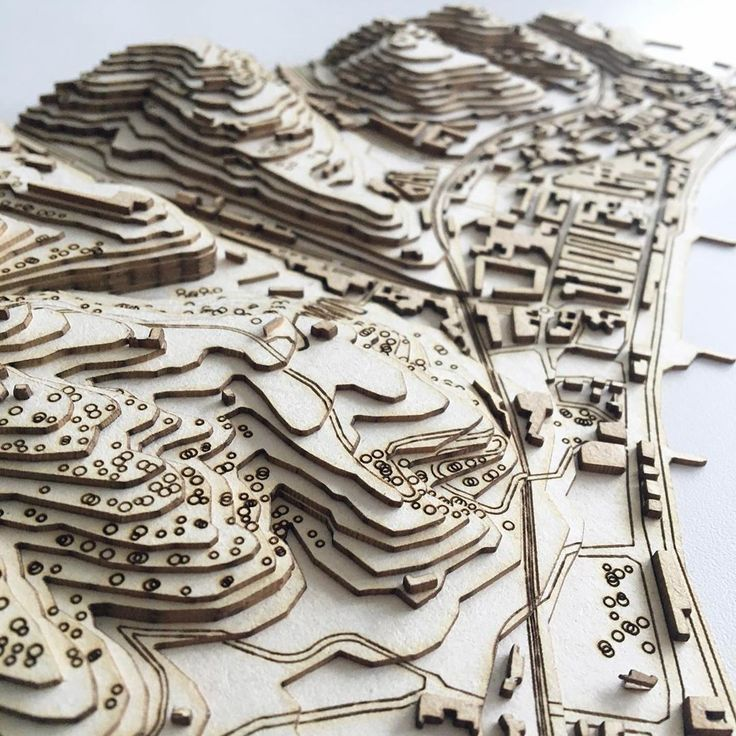
\includegraphics[width=0.7\textwidth]{chapters/120-topologie/images/relief.jpg}
\caption{Rekonstruktion einer Approximation der Topographie aus den
\index{Topographie}%
Höhenlinien mit Hilfe von Platten, die entlang der Höhenlinien ausgeschnitten
worden sind.
\label{buch:topologie:morse:fig:relief}}
\end{figure}
%
Aus einer glatten Funktion $f\colon M\to\mathbb{R}$ lässt
sich eine natürliche Zerlegung einer Mannigfaltigkeit konstruieren.
In Abbildung~\ref{buch:topologie:morse:fig:karte} zeigt eine 
topographische Karte.
Die Höhenlinien sind die Niveaulinien der Funktion, die einem
Punkt seine Höhe über dem Meeresspiegel zuordnet.
Die Höhenlinien zerlegen die Karte in Streifen, Ringe und andere
zweidimensionale Gebiete.
Der geübte Kartenleser ist in der Lage, aus den Höhenlinien eine
Vorstellung der Topographie zu rekonstruieren.
Man kann aber auch aus den Höhenlinien ein massstäbliches Modell
des Geländes rekonstruieren.
Für jedes Niveau schneidet man das von der Höhenlinie berandete Gebiet
aus einer Holzplatte aus und schichtet die erhaltenen Platten
wie in Abbildung~\ref{buch:topologie:morse:fig:relief} gezeigt
auf.
Es entsteht eine Approximation des Geländes.

Wir betrachten jetzt eine einzelne Höhenlinie.
Die Höhenlinie zur Höhe $c$ ist die Menge der Punkte
\[
H_c
=
\{ p\in M\mid f(p) = c \}.
\]
Wenn wir $c$ um einen kleinen Betrag $\Delta c$ verschiebt sich
die Höhenlinie in eine Richtung senkrecht auf die Höhenlinie.
Ein positives $\Delta c$ bedeutet, dass wir eine Höhenlinie weiter
oben am Berg suchen.
Ist $\Delta c$ klein genug, ist die neue Höhenlinie $H_{c+\Delta c}$
meistens eine Kurve, die in unmittelbarer Nähe der Kurve $H_c$.
die Veränderung von $c$ hat also keine wesentlichen Auswirkungen
auf die Gestalt der Höhenlinie, wenigstens wenn die Höhenlinie
immer an einem Hang entlang verläuft.

Die Voraussetzung, dass die Höhenlinie dem Hang entlang verlaufen
muss, damit einen kleine Höhenänderung keine Auswirkung auf die
Gestalt der Kurve hat, ist zum Beispiel bei einem Gipfel verletzt.
Sei $p$ ein lokales Maximum der Funktion $f$ und U eine so kleine
Umgebung von $p$, dass die Höhenlinie $H_c = \{p\}$ nur den Punkt $p$
enthält.
Vergrössert man $c$ um $\Delta c>0$, verschwindet der Punkt $p$,
die Höhenlinie $H_{c+\Delta c}=\emptyset$ ist leer.
Bei einer Verkleinerung wird wird die Höhenline $H_{c+\Delta c}$ zu
einer geschlossenen Kurve, die den Punkt $p$ umschliesst
(Abbildung~\ref{buch:topologie:morse:fig:karte}, Umgebung des Punktes 1384),
wenigstens wenn die zweiten Ableitungen von $f$ an der Stelle $p$
nicht verschwinden.

Ein ganz anderes Bild bietet sich bei einem Pass der Höhe $c$.
Auch ein Sattelpunkt der Fläche ist eine Stelle, an der
alle partiellen ersten Ableitungen verschwinden.
Die Menge $H_c$ besteht aber nicht aus einem Punkt, vielmehr
kommen im Punkt $p$ vier Höhenlinien zusammen.
Für grössere und kleiner Werte verschwindet der Schnittpunkt,
es bleiben zwei nicht verbundene Höhenlinie wie in
bei links unterhalb der Büelhöchi in
Abbildung~\ref{buch:topologie:morse:fig:karte}.

Diese Diskussion zeigt, dass wesentliche Eigenschaften der Topographie
aus Punkten abzulesen sind, an denen die ersten Ableitungen verschwinden,
die zweiten Ableitungen aber nicht (was das genau heisst, muss noch
definiert werden).

%
% Index einer Nullstelle
%
\subsection{Kritische Punkte und ihr Index}
In diesem Abschnitt ist $M$ eine $n$-dimensionale Mannigfaltigkeit.
Wir betrachten die Menge $C^\infty(M)$ der beliebig oft stetig
differenzierbare Funktionen auf $M$.

%
% Kritische Punkte
%
\subsubsection{Kritische Punkte}
%
% fig-morse.tex
%
% (c) 2025 Prof Dr Andreas Müller
%
\begin{figure}
\centering
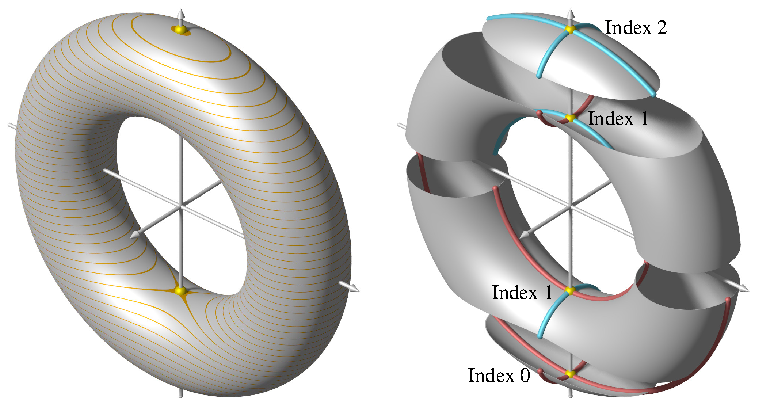
\includegraphics{chapters/120-topologie/images/morse.pdf}
\caption{Links: Torus mit Höhenlinien der Funktion $f(p) = z(p)$ für Punkte
$p$ auf dem Torus.
\index{Torus}%
Kritische Punkte von $f$ sind gelb eingezeichnet.
\index{kritischer Punkt}%
Rechts: Der Torus lässt sich in Teile zerlegen, die jeweils genau
einen kritischen Punkte enthalten. Aus den Indizes der kritischen Punkte
\index{Index}%
lassen sich topologische Eigenschaften der Mannigfaltigkeit rekonstruieren.
\label{buch:topologie:fig:morse}}
\end{figure}
%
Die äussere Ableitung einer Funktion $f\colon M\to\mathbb{R}$ 
wird ein einer Karte $\varphi_\alpha\colon U_\alpha\to\mathbb{R}^n$
zu einer Funktion der $n$ Koordinaten, die wir $f(x^1,\dots,x^n)$
schreiben.
Bei einem Maximum oder Minimum der Funktion verschwinden alle ersten
Ableitungen, in dieser Karte wird die äussere Ableitung
\[
df
=
\frac{\partial f}{\partial x^1}\,dx^1
+
\dots
+
\frac{\partial f}{\partial x^n}\,dx^n
=
0.
\]
Wechselt man das Koordinatensystem, ändert dies an der Tatsache, dass
$df=0$ ist, nichts.

\begin{definition}[kritischer Punkt]
\index{kritischer Punkt}%
\index{Punkt!kritisch}%
\index{kritischer Wert}%
\index{Wert!kritisch}%
Ein \emph{kritischer Punkt} einer glatten Funktion $f$ auf einer
differenzierbaren Mannigfaltigkeit ist ein Punkt $p\in M$, bei dem
$df(p)=0$ ist.
Der Wert $c=f(p)$ in einem kritischen Punkt $p$ heisst
\emph{kritischer Wert} der Funktion f.
\end{definition}

%
% Der Index eines kritischen Punktes
%
\subsubsection{Der Index eines kritischen Punktes}
Sei $p$ ein kritischer Punkt der Funktion $f$ auf der Mannigfaltigkeit $M$
mit dem kritischen Wert $c=f(p)$.
In einem Koordinatensystem in der Umgebung des Punktes $p$ kann die Funktion
durch die Taylor-Reihe 
\begin{align}
f(x^1,\dots,x^n)
&=
f(p)
+
\sum_{k=1}^n \frac{\partial f}{\partial x^k}(p) (x^k-x^k(p))
\\
&\qquad\mathstrut
+
\sum_{k,l=1}^n
\frac{\partial^2 f}{\partial x^k\,\partial x^l}(p)
(x^k-x^k(p))(x^l-x^l(p))
+
o(|x-p|^2)
\notag
\\
&=
c
+
\sum_{k,l=1}^n
\frac{\partial^2 f}{\partial x^k\,\partial x^l}(p)
(x^k-x^k(p))(x^l-x^l(p))
+
o(|x-p|^2)
\label{buch:topologie:morse:eqn:quadratisch}
\end{align}
approximiert werden.
Wir möchten sicherstellen, dass wir zuverlässige Aussagen über die
Form der \emph{Niveaumengen} $H_c=\{p\in M\mid f(p)=c\}$ machen können.
Dazu muss der quadratische Term in
\eqref{buch:topologie:morse:eqn:quadratisch}
immer gegenüber den Termen höherer Ordnung dominieren.
Dies ist nur möglich, wenn der quadratische Ausdruck
\[
H(v)
=
\sum_{k,l=1}^n
\frac{\partial^2 f}{\partial x^k\,\partial x^l}
v^k v^l
\]
nicht entartet ist.

\begin{definition}[entartete quadratische Form]
XXX
\end{definition}

Die Matrix $H$ mit den Einträgen
\[
h_{kl} = \frac{\partial^2 f}{\partial x^k\,\partial x^l}
\]
ist in einem nicht entarteten kritischen Punkt eine symmetrische
Matrix.
Da symmetrische Matrizen durch orthogonale Transformationen
diagonalisierbar sind, können wir das Koorinatensystem mit
einer orthogonalen Matrix so drehen, dass $H$ die Form
\[
H(v)
=
\sum_{i=1}^n \lambda_i (v^i)^2
\]
bekommt.
Die $\lambda_i$ sind die Eigenwerte der Matrix $H$, keiner
der Eigenwerte verschwindet.
Durch Streckung der Koordinatenachse $x^1$ mit dem Faktor
$\!\sqrt{|\lambda_i|}$  mittels
$y^i = \!\sqrt{|\lambda_i|}x^i$ kann die Entwicklung
\eqref{buch:topologie:morse:eqn:quadratisch}
in die Form
\begin{align*}
f(y^1,\dots,y^n)
&=
c
+
\operatorname{sgn}(\lambda_1)\,(y^1)^2
+
\dots
+
\operatorname{sgn}(\lambda_n)\,(y^n)^2.
\end{align*}
Es kommt also nur auf die Vorzeichen der Eigenwerte an.
Bei einem Koordinatenwechsel ändert sich die Matrix $H$ der zweiten
Ableitungen, aber die Anzahl der positiven und negativen Eigenwerte
bleibt erhalten.

\begin{definition}[Index]
\index{Index einer quadratischen Form}%
Der \emph{Index} einer nicht entarteten quadratischen Form ist die
Anzahl der negativen Eigenwerte.
\end{definition}

%
% Rekonstruktion
%
\subsection{Rekonstruktion}

%
% de Rham Kohomologie
%
\section{de Rham-Kohomologie}

\subsection{Zyklen und Ränder}

\subsection{Definition der Kohomologiegruppen}

%
% Beispiele
%
\subsection{Beispiele}

\subsubsection{Zusammenziehbarer Raum}

\subsubsection{Torus}

\subsubsection{Kugel}

